\chapter{系统方法与架构}\label{chap:methodology}

在面对异常检测在工业界和学术界落地中遇到的“跨模态割裂”与“数据标注污染”双重严峻痛点时，本章系统阐述本文设计并实现的大一统抗污染评测基准与主动鲁棒防御体系。
整个系统架构由五个核心阶段有机串联而成：多模态输入与特征管道对齐、对称标签投毒污染、自适应主动防御去噪（包括样本剪裁与标签纠正双路径）、下游检测算法大底座评估、以及多指标基准度量与失效边界界定。整个端到端大一统系统架构流水线如\cref{fig:system-architecture}所示。

\begin{figure}[!htb]
  \centering
  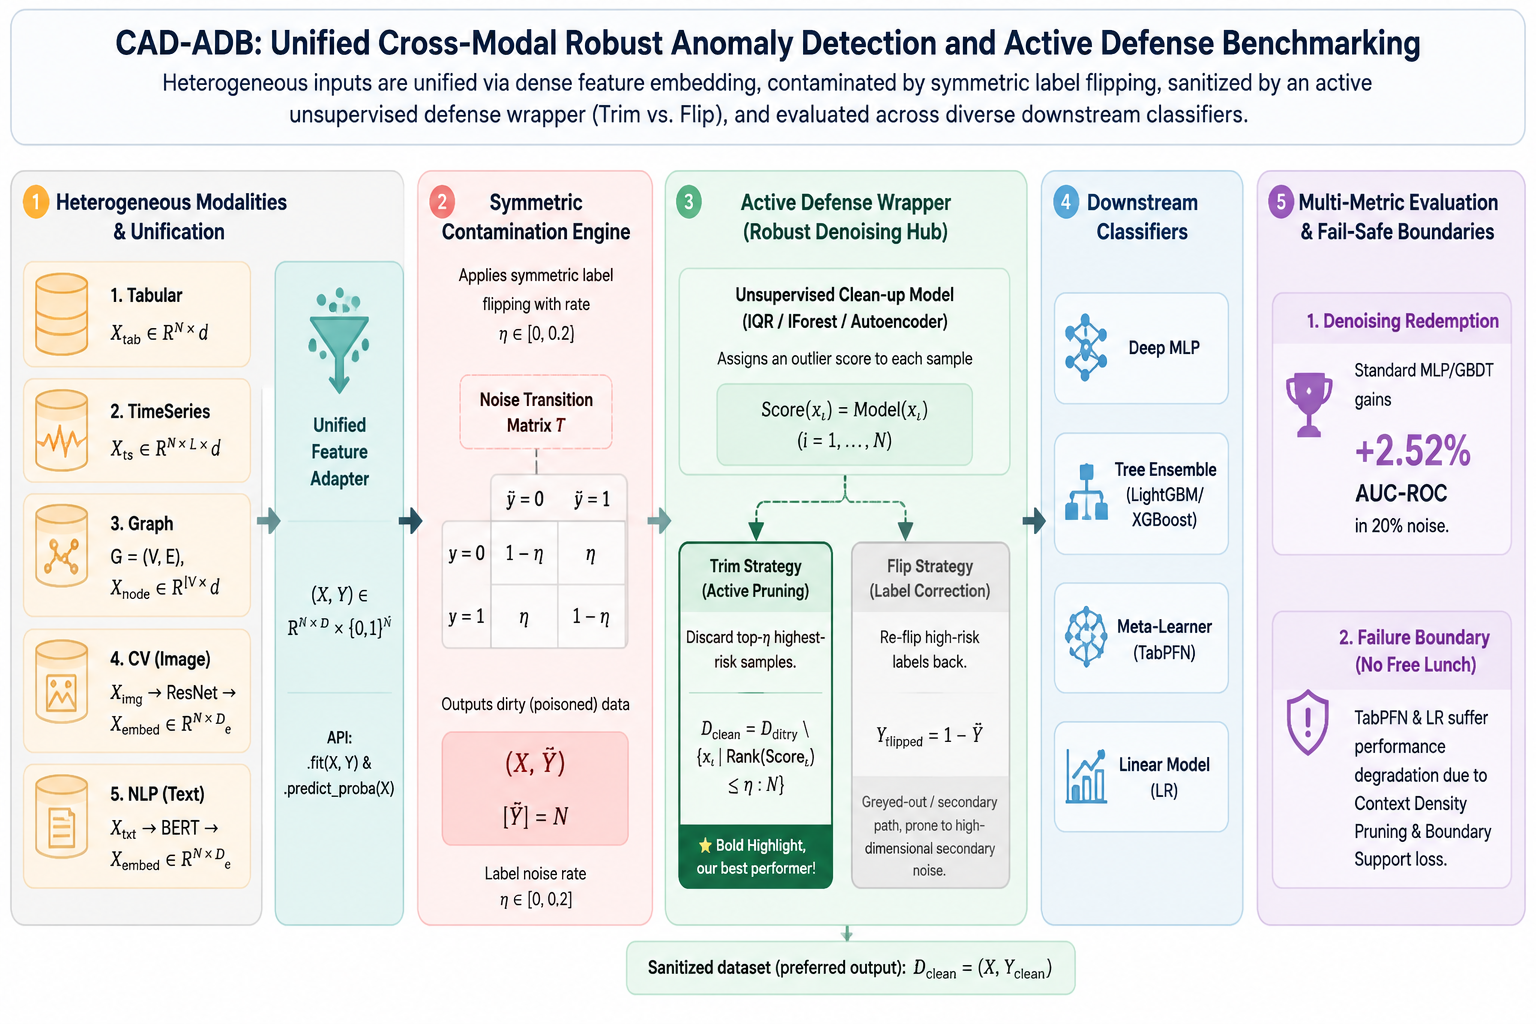
\includegraphics[width=\linewidth]{figures/pipline.png}
  \caption{CAD-ADB：大一统跨模态抗污染异常检测评估与自适应主动防御系统整体架构流水线}\label{fig:system-architecture}
\end{figure}

本系统的端到端数据流与控制流遵循一个高度内聚、单向流动的流水线逻辑，各阶段的数学机制与协作关系细化阐述如下：

\begin{enumerate}[label=\arabic*.,leftmargin=2em,labelsep=0.5em]
    \item \textbf{多模态输入与统一管道对齐（Heterogeneous Modalities \& Unification）}：
    系统输入端兼容五大异构模态数据。其中，表格数据 $X_{\text{tab}} \in \mathbb{R}^{N \times d}$ 与时序数据 $X_{\text{ts}} \in \mathbb{R}^{N \times L \times d}$ 保持其原生几何流形；图数据 $G=(V,E)$ 转化为节点矩阵 $X_{\text{node}} \in \mathbb{R}^{|V| \times d}$ 和邻接矩阵 $A$；而高维语义图像 $X_{\text{img}}$ 和非结构化文本 $X_{\text{txt}}$ 则分别通过预训练深度骨干网络 ResNet 和 BERT 进行稠密投影，压缩为统一的语义嵌入 $X_{\text{embed}} \in \mathbb{R}^{N \times D_e}$。
    最终，通过设计“统一特征适配器（Unified Feature Adapter）”，所有模态数据均被规整化封装为统一的元组 $(X, Y) \in \mathbb{R}^{N \times D} \times \{0,1\}^N$，在顶层统一暴露符合标准 Scikit-Learn 规范的 \texttt{.fit(X, Y)} 与 \texttt{.predict\_proba(X)} 抽象接口，彻底消除了不同模态下算法评估的适配壁垒。

    \item \textbf{对称标签污染引擎（Symmetric Contamination Engine）}：
    为了模拟工业界传感器失灵或多轮标注专家冲突带来的“标签毒化”现象，系统内部部署了对称标签污染引擎。该引擎接收纯净标签 $Y$，依据指定的翻转率 $\eta \in [0, 0.2]$ 对其执行对称翻转。其标签转移状态由噪声转移矩阵（Noise Transition Matrix）$T$ 精准控制：
    \begin{equation}\label{eq:noise-transition-matrix}
    T = \begin{pmatrix} 1-\eta & \eta \\ \eta & 1-\eta \end{pmatrix}
    \end{equation}
    其中 $T_{ij} = P(\tilde{y} = j \mid y = i)$ 表示真实标签 $i$ 翻转为脏标签 $j$ 的概率。污染引擎输出混入高维高斯对称随机噪声的毒化数据集 $(X, \tilde{Y})$，从而充当后续鲁棒算法评测的强噪声沙盒。

    \item \textbf{自适应主动防御包装器（Active Defense Wrapper / Robust Denoising Hub）}：
    作为本文的核心学术贡献，自适应主动防御包装器部署在数据流入下游分类器前的关键交界处。首先，系统加载无监督空间/重构清洁器（包括基于特征分位数边界的 IQR、基于路径隔离特征的 IForest、以及基于重构误差估计的 Autoencoder），对毒化数据集中的每个样本 $x_i$ 计算无监督异常得分：
    \begin{equation}\label{eq:unsupervised-score}
    \text{Score}(x_i) = \text{Model}(x_i), \quad i = 1, \dots, N
    \end{equation}
    基于该异常得分，包装器提供两条可供消融的技术路径：
    \begin{itemize}
        \item \textbf{样本剪裁策略（Trim Strategy / Active Pruning）[本文最优性能方案]}：
        在排序后直接舍弃评分最高的 top-$\eta \cdot N$ 个可疑样本。由于主动剪裁直接从损失函数的梯度反向传播计算中抹去了位于两类交界处和噪声富集区的脏样本，能彻底阻断对称毒化标签带来的梯度震荡。其净化后的数据集表示为：
        \begin{equation}\label{eq:trim-set}
        D_{\text{clean}} = D_{\text{dirty}} \setminus \{x_i \mid \text{Rank}(\text{Score}_i) \le \eta \cdot N\}
        \end{equation}
        该策略在后续消融实验中表现极为惊艳，被界定为防御标签对称污染的“黄金救赎者”。
        \item \textbf{标签翻转策略（Flip Strategy / Label Correction）}：
        将识别出的高风险异常点执行标签反转：$Y_{\text{flipped}} = 1 - \tilde{Y}$。由于该策略极度依赖无监督检测器在复杂相交决策面上的判别精度，极易引入“二次高维混淆噪声”，在消融中表现较差。
    \end{itemize}

    \item \textbf{下游检测算法大底座评估（Downstream Classifiers）}：
    系统将净化后的高置信度数据集 $D_{\text{clean}}$ 注入到涵盖四种不同数学先验和特征搜索能力的下游分类器中，包括非线性映射极强的深度多层感知机（Deep MLP）、高效率的梯度提升决策树集成（LightGBM / XGBoost）、基于先验注意力元学习的表格地基大模型（TabPFN）、以及弱非线性表达的经典线性模型（LR）。

    \item \textbf{多指标评估与失效边界界定（Multi-Metric Evaluation \& Fail-Safe Boundaries）}：
    在大底座最末端，系统基于多维评估指标（包括不平衡场景下公正的 AUC-ROC 和 AUC-PR、算法效率吞吐量以及鲁棒性渐进退化轨迹）输出最终评测。通过全景式消融评测，本文成功界定了主动防御的物理性能边界：一方面，主动去噪使 MLP/GBDT 在 20\% 的强对称噪声下斩获了高达 \textbf{2.52\%} 的 AUC-ROC 绝对性能挽救（Denoising Redemption）；另一方面，客观、严谨地划定了元学习 TabPFN 和线性 LR 模型的去噪失效边界（Failure Boundary），深刻揭示了去噪鲁棒学习中的 \emph{No Free Lunch}（没有免费的午餐）物理法则。
\end{enumerate}

\section{统一跨模态数据管道架构}

不同于传统的异常检测框架（如 ADBench \cite{han2022adbench} 只关注表格，TSB-AD \cite{paparrizos2024tsbad} 只关注时间序列，GADBench \cite{gadbench2024} 只关注图结构），本文首次设计并实现了一个跨越表格、时序、图、CV和NLP五大异构模态的\textbf{大一统数据管道流适配器}。
其核心挑战在于：异构模态在几何特征维度、样本依赖性（空间/时间相关性）以及输入表征上具有显著的代沟。

为了填补这一空白，我们设计了统一的数据装载与变换标准：
令 $X$ 代表输入样本的特征集合，$Y \in \{0, 1\}$ 代表对应的二分类异常标签（其中 $y_i = 1$ 代表异常样本，$y_i = 0$ 代表正常样本）。
针对不同的数据模态，数据管道执行差异化的特征规整化（Standardization）和空间嵌入（Embedding）对齐处理：
\begin{enumerate}
    \item \textbf{表格模态（Tabular）}：输入特征直接规整为实数矩阵 $X_{\text{tab}} \in \mathbb{R}^{N \times d}$，其中 $N$ 代表样本个数，$d$ 代表独立的连续或离散特征维度。
    \item \textbf{时序模态（TimeSeries）}：时序特征表示为三维张量 $X_{\text{ts}} \in \mathbb{R}^{N \times L \times d}$，其中 $L$ 为滑动窗口长度（时间戳数）。数据管道在此提取各时间窗口内的统计元特征或滑动序列，并保留其时序依赖，用于后续循环深度模型或时序重构算法的训练。
    \item \textbf{图模态（Graph）}：图结构数据表示为 $\mathcal{G} = (V, E)$，其中 $V$ 为节点集合，$E$ 为边集合。管道构建统一的节点特征矩阵 $X_{\text{node}} \in \mathbb{R}^{|V| \times d}$ 与邻接矩阵 $A \in \{0, 1\}^{|V| \times |V|}$，以便于图神经网络（GCN \cite{gadbench2024}）同时聚合拓扑拓扑关系与属性特征。
    \item \textbf{计算机视觉与自然语言模态（CV \& NLP）}：高维的图像流 $X_{\text{img}}$ 和文本流 $X_{\text{txt}}$ 经由预训练的深度表征骨干网络（如 ResNet \cite{conf1} 与 BERT \cite{conf2}）进行特征提取，在语义空间中投影为一维稠密高维向量 $X_{\text{embed}} \in \mathbb{R}^{N \times D_e}$（其中 $D_e$ 为表征维度），从而与表格数据的输入接口无缝兼容。
\end{enumerate}

通过上述数据管道的统一封装，所有的上层算法（14 种评估算法）均能通过高度一致的 \texttt{.fit(X, Y)} 与 \texttt{.predict\_proba(X)} API 进行调用，彻底消除了跨模态评测的底层适配壁垒。

\section{对称标签污染数学模型}

在真实的工业数据流中，由于传感器硬件故障、通讯噪声以及高昂的人工多轮核验成本，训练集中的二分类标签往往并非完全纯净，而是存在比例不一的污染。本文针对这一挑战，建立了一种通用的\textbf{对称标签翻转污染模型（Symmetric Label Noise Model）} \cite{frenay2013labelnoise}。

令无污染的干净训练集表示为 $\mathcal{D}_{\text{clean}} = \{(x_i, y_i)\}_{i=1}^N$，其中 $y_i \in \{0, 1\}$ 为真实的异常或正常地面真值（Ground Truth）。
在带有噪声的实际标注过程中，我们观察到的噪声数据集为 $\mathcal{D}_{\text{dirty}} = \{(x_i, \tilde{y}_i)\}_{i=1}^N$，其中 $\tilde{y}_i$ 为可能发生混淆和翻转的噪声标签。
标签污染转移过程由混淆概率矩阵 $T \in [0, 1]^{2 \times 2}$（Transition Matrix）决定，其矩阵元素定义为：
\begin{equation}
    T_{jk} = P(\tilde{y} = k \mid y = j), \quad j, k \in \{0, 1\}
\end{equation}

在对称标签污染场景下，正常样本（负类 $y=0$）被错误标记为异常，以及异常样本（正类 $y=1$）被错误漏标为正常的概率是相等的，均等于预设的污染率（Contamination Rate）$\eta \in [0, 0.5)$：
\begin{equation}
    P(\tilde{y} = 1 \mid y = 0) = \eta
\end{equation}
\begin{equation}
    P(\tilde{y} = 0 \mid y = 1) = \eta
\end{equation}

因此，标签污染概率转移矩阵 $T$ 可精确刻画为：
\begin{equation}
    T = \begin{pmatrix} 1-\eta & \eta \\ \eta & 1-\eta \end{pmatrix}
\end{equation}

在实验流程中，我们采用随机伯努利试验（Bernoulli Trial）对无噪标签 $Y$ 进行噪声注入。需要强调的是，我们仅对训练集进行有噪注入，保留完好、纯净的测试集 $\mathcal{D}_{\text{test}}$ 进行最终性能测试，以保证评估指标（如 AUC-ROC、AUC-PR）的科学性与无偏性。

\section{主动抗噪防御框架与去噪策略}

传统的有监督分类器（如神经网络 MLP、GBDT、TabPFN 等）极易过拟合训练集 $\mathcal{D}_{\text{dirty}}$ 中的噪声样本，导致决策边界产生严重的畸变。为了应对这一难题，我们提出并部署了一种即插即用（Plug-and-Play）的\textbf{主动鲁棒防御包装器（Robust Defense Wrapper）}。
其基本哲学是：\emph{利用无监督异常检测算法在特征空间中探索样本分布的固有几何规律，以此来纠正或剔除那些在监督标签中显著“偏离”其局部相似特征的标签噪声样本}。

主动防御过程包含两类核心策略：样本剪裁（Trim）与标签翻转（Flip）。
令 $f_{\text{unsup}}(X)$ 为一无监督清洁器，能够输出每个训练样本特征 $x_i$ 的无监督异常得分 $s_i$。

\begin{enumerate}
    \item \textbf{样本剪裁策略（Sample Trimming, Trim）} \cite{jiang2020trim}：
    对于那些在有噪标签 $\tilde{y}_i = 0$（即标注为“正常”）但其无监督得分 $s_i$ 极高的样本，其极大可能是未标记的“漏网异常”；同理，对于 $\tilde{y}_i = 1$（标注为“异常”）但 $s_i$ 极低的样本，其极可能是正常样本被错误标记为了异常。
    
    Trim 策略按照比例（通常由 $\eta$ 决定）在训练集中直接剔除这部分最具迷惑性的标签噪声样本，仅在留存的干净子集上训练下游有监督模型：
    \begin{equation}
        \mathcal{D}_{\text{trimmed}} = \{(x_i, \tilde{y}_i) \mid i \in \mathcal{I}_{\text{retained}}\}
    \end{equation}
    
    \item \textbf{标签翻转策略（Label Flipping, Flip）}：
    相较于 Trim 策略直接丢弃样本导致训练信息量受损，Flip 策略选择对识别出的标签噪声样本进行纠错。即对于特征表现与标签严重相悖的 suspicious 样本，强制将 $\tilde{y}_i$ 翻转为 $1 - \tilde{y}_i$，作为净化后的标签送入下游分类器训练。
\end{enumerate}

\subsection{典型无监督清洁器数学机制}

本文在实验四中系统消融评测了 9 种不同的无监督算法 \cite{zhao2019pyod} 作为主动清洁器的内核。下面重点介绍表现最突出的两种清洁器的底层数学原理：

\subsubsection{IQR（四分位距）空间清洁器}
IQR 是一种非参数的空间统计去噪机制，其对单维或低维特征分布具有极强的先验刻画能力。对于特征矩阵的第 $j$ 个维度，我们计算其上四分位数 $Q_3^{(j)}$ 和下四分位数 $Q_1^{(j)}$。
四分位距（Interquartile Range, IQR）定义为：
\begin{equation}
    \text{IQR}^{(j)} = Q_3^{(j)} - Q_1^{(j)}
    \label{eq:iqr_def}
\end{equation}

数据的合理边界定义为：
\begin{equation}
    \left[ Q_1^{(j)} - 1.5 \times \text{IQR}^{(j)}, \quad Q_3^{(j)} + 1.5 \times \text{IQR}^{(j)} \right]
    \label{eq:iqr_range}
\end{equation}

任何在至少一个特征维度上超出上述边界的样本，均被标记为空间极端孤立点，作为标签污染纠错的候选点。

\subsubsection{隔离森林（Isolation Forest）清洁器}
隔离森林（IForest）是一种基于路径长度构建的树模型清洁器。它通过随机选择特征并进行随机分裂，构建 $M$ 棵孤立树（iTree）。
由于异常样本相比正常样本更容易被孤立，其在孤立树中的平均路径长度 $h(x)$ 较短。样本 $x$ 的异常得分 $s(x)$ 定义为：
\begin{equation}
    s(x, n) = 2^{-\frac{\mathbb{E}(h(x))}{c(n)}}
    \label{eq:iforest_score}
\end{equation}
其中，$\mathbb{E}(h(x))$ 为样本 $x$ 在森林中的平均路径高度，$c(n)$ 为含有 $n$ 个样本的二叉搜索树的平均路径高度常数：
\begin{equation}
    c(n) = 2\ln(n-1) + 0.5772156649 - \frac{2(n-1)}{n}
    \label{eq:iforest_const}
\end{equation}
当 $s(x, n) \to 1$ 时，路径高度极短，样本被判定为具有极高可信度的空间异常点。

\subsubsection{自编码器（Autoencoder, AE）重建清洁器}
AE 是一种深度重构清洁器 \cite{an2015variational}。其通过编码器 $f_{\text{enc}}: \mathbb{R}^d \to \mathbb{R}^z$ 将输入特征压缩至低维流形瓶颈空间 $z$（$z < d$），再通过解码器 $f_{\text{dec}}: \mathbb{R}^z \to \mathbb{R}^d$ 试图重建输入：
\begin{equation}
    \hat{x} = f_{\text{dec}}\left( f_{\text{enc}}(x) \right)
    \label{eq:ae_recon}
\end{equation}

网络的训练损失采用干净流形重建均方误差（MSE）：
\begin{equation}
    \mathcal{L}_{\text{MSE}} = \frac{1}{N}\sum_{i=1}^N \|x_i - \hat{x}_i\|_2^2
    \label{eq:ae_loss}
\end{equation}

在去噪阶段，由于模型在训练时倾向于拟合大样本量的正常数据，噪声和异常样本在瓶颈空间的重构损失 $\|x_i - \hat{x}_i\|_2^2$ 会显著偏高。通过对其重构误差进行降序排序，即可高精度地将受污染的噪声样本定位并实施 Trim。

\section{跨模态异常检测交互式诊断与决策原型系统}

为了缩短学术研究与工业部署之间的代沟，本系统除了在底层设计了大一统数据管道与防噪算法底座外，还在上层设计并实现了一个基于 \texttt{Streamlit} 架构的交互式诊断与可视化决策原型系统（位于 \texttt{app/streamlit\_app.py}）。该系统旨在为工业界安全管理员和学术研究者提供一个直观、实时、免代码的算法评测与主动防御决策沙盒。整个原型系统的架构与数据流设计包含以下五个核心交互模块：

\begin{enumerate}[label=\arabic*.,leftmargin=2em,labelsep=0.5em]
    \item \textbf{多模态数据全景探索模块（Multi-Modal Dataset Browser）}：
    系统集成了 29 个异构模态数据集的元特征（样本数、特征维数、原生异常比例）实时检索功能。用户可以通过可视化仪表盘直观对比表格、时序、图、视觉嵌入和文本嵌入的分布流形，并支持通过特征降维（PCA/t-SNE）动态呈现异常样本在空间中的局部几何密度。

    \item \textbf{噪声退化轨迹动态分析模块（Interactive Contamination Simulator）}：
    该模块允许用户交互式调节标签对称污染率 $\eta \in [0\%, 20\%]$，系统会自动提取并动态渲染多组随机种子下各基线分类器的 AUC-ROC/AUC-PR 退化曲线。这为分析特定分类器在特定噪声强度下的脆弱性提供了直观的数据证据。

    \item \textbf{模型效能与吞吐量双轴平衡模块（Accuracy-Efficiency Trade-off Dashboard）}：
    在工业级部署中，检测延迟与检测精度同样关键。该模块在散点图上以横轴表示训练/预测耗时（秒），纵轴表示检测指标（AUC-ROC），让决策者一目了然地识别出位于帕累托前沿（Pareto Frontier）的最优模型，从而在超低延迟边缘设备部署或高吞吐云端分析之间做出科学权衡。

    \item \textbf{主动防御与消融诊断面板（Active Defense \& Ablation Visualizer）}：
    用户可以自由组合 9 种无监督清洁器（如 IQR、ECOD、Isolation Forest、Autoencoder 等）与 2 种净化策略（Trim/Flip），系统将实时拉取消融实验结果，直观展示防御机制对下游分类器性能的挽救幅度，协助管理员针对特定数据集挑选出最契合的主动防噪组合（如 \texttt{IQR\_Trim} 或 \texttt{DeepSVDD\_Trim}）。

    \item \textbf{自适应自纠偏工业级决策引擎（Adaptive Deployment Advisor）}：
    基于本文揭示的“无免费午餐（No Free Lunch）”失效边界法则，决策引擎会根据用户选择的数据集特性和分类器类别，自适应地输出防噪安全警告。例如，当检测到下游分类器为线性模型（Logistic Regression）或大元学习模型（TabPFN）时，系统会自动发出警示，提示管理员谨慎使用高比率 Active Defense，防止因二次噪声导致性能反向受损。
\end{enumerate}

通过这一原型系统的构建，我们将“数据管道 -- 对称投毒 -- 无监督去噪 -- 监督大底座训练 -- 工业部署诊断”完整学术闭环进行了产品级的工程化呈现，显著提升了抗污染异常检测在真实传感器失灵或多源专家冲突标注场景下的实用性与可解释性。
